\chapter{Introduction}

The increasing adoption of Artificial Intelligence techniques in embedded and
resource-constrained systems has highlighted the importance of efficient
software--hardware co-design methodologies.
In particular, the deployment of Deep Neural Networks (DNNs) on embedded platforms
poses significant challenges in terms of computational complexity, memory usage,
data movement, and real-time constraints.

This laboratory activity (Lab~5) builds upon the concepts and methodologies
introduced in Laboratory~3 and Laboratory~4, extending low-level performance
measurement and software optimization techniques to the implementation of a
complete DNN inference pipeline.
While previous laboratories focused on isolated computational kernels
(e.g., FIR filtering and parallel vector operations), this work addresses the
integration of computation, communication, and performance profiling within a
single embedded application.

The report describes the implementation of a DNN-based microserver for handwritten
digit recognition (MNIST) running on the Zybo Z7 platform.
The application performs real-time inference on images streamed from a host PC via
UART and is specifically designed according to embedded system constraints,
without relying on hardware accelerators or dedicated neural processing units.

The target platform is based on the Zynq-7000 System-on-Chip, where an ARM Cortex-A9
Processing System executes a fully software-based inference pipeline.
The adopted approach emphasizes explicit control over data representation,
memory organization, and execution flow, which are key aspects in the context of
Advanced Embedded Systems.

The implemented DNN processes grayscale images of size $28 \times 28$ pixels and
classifies each input sample as a digit in the range from 0 to 9.
Inference is carried out using fixed-point arithmetic, allowing the elimination of
floating-point operations and ensuring deterministic execution behavior.
Multiple fixed-point configurations are supported and selected at compile time,
including a baseline reference configuration and optimized modes targeting
communication efficiency and numerical robustness.

In addition to functional correctness, particular attention is devoted to the
experimental evaluation of performance.
Execution times are measured using the ARM Cortex-A9 Global Timer through the
\texttt{XTime\_GetTime()} API, enabling fine-grained profiling of individual stages
such as UART-based data reception, fully connected layers, activation functions,
and result processing.
This measurement-driven approach allows a quantitative assessment of real-time
capability and highlights the impact of system-level optimizations.

Finally, the report presents an extended implementation based on a custom DNN
topology assigned to Group~4, demonstrating the scalability and modularity of the
proposed software framework.
The combination of architectural analysis, fixed-point design, and experimental
profiling provides a comprehensive view of how DNN inference can be effectively
mapped onto an embedded ARM-based platform under realistic I/O and performance
constraints.


\chapter{Target Platform and Development Environment}

The target platform for this laboratory activity is the Processing System (PS)
of the Zynq-7000 System-on-Chip, specifically the ARM Cortex-A9 core available on
the Zybo Z7 development board.
The Zynq-7000 architecture integrates a dual-core ARM processing system with
programmable logic on the same device, enabling a wide range of hardware--software
co-design solutions.

In this work, the entire Deep Neural Network inference pipeline is executed
exclusively on the ARM Cortex-A9 processor, without exploiting the programmable
logic or any dedicated hardware accelerator.
This design choice is deliberate and aligns with the objectives of the laboratory,
which focus on evaluating software efficiency, fixed-point arithmetic, and
performance profiling under embedded constraints.
By avoiding hardware acceleration, the implementation allows direct analysis of
instruction-level execution, memory access patterns, and real-time behavior on a
general-purpose embedded processor.

The software is developed as a standalone application using the Xilinx Software
Development Kit (SDK).
The standalone execution model avoids the overhead introduced by an operating
system, providing direct access to hardware peripherals and enabling precise and
deterministic timing measurements.
This execution environment is particularly suitable for low-level optimization and
performance evaluation tasks, which are central topics in the Advanced Embedded
Systems course.

\begin{figure}[H]
    \centering
    
\includegraphics[width=0.65\textwidth]{images/xilink}
    \caption{Xilinx Software Development Kit (SDK) environment used for embedded application development.}
    \label{fig:xilinx_sdk}
\end{figure}

Communication between the host computer and the embedded platform is implemented
through a UART interface.
The UART channel is used to stream MNIST input images from the host PC to the board
and to transmit classification results back to the host.
This communication model reflects a realistic embedded scenario, where external
data sources are often connected through low-bandwidth serial interfaces.
The use of UART also enables clear separation between communication latency and
computation time, which is essential for meaningful performance analysis.

\begin{figure}[H]
    \centering
    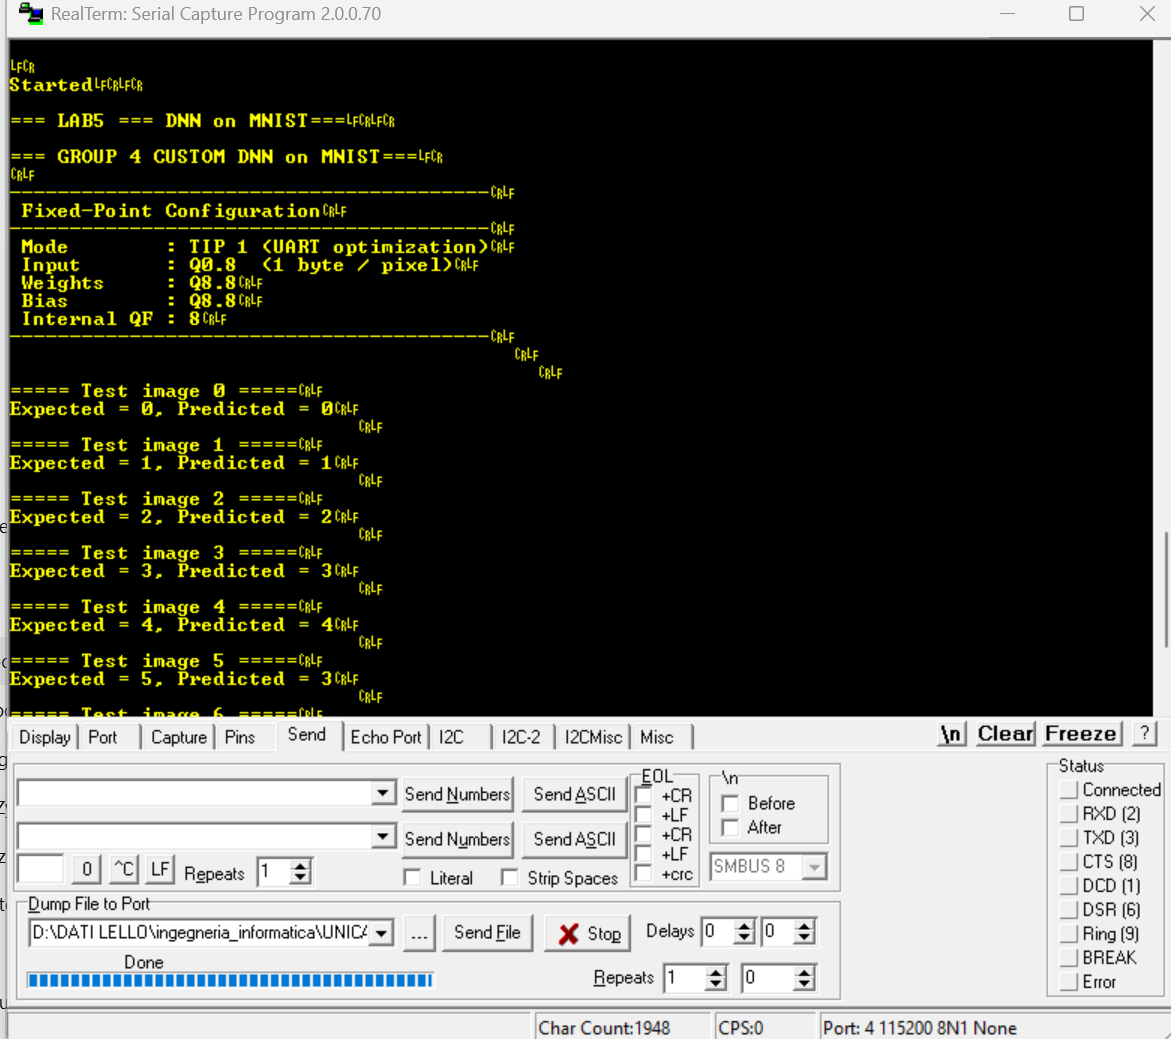
\includegraphics[width=0.75\textwidth]{images/tip1 stampa}
    \caption{RealTerm serial/TCP terminal used to transmit binary MNIST data streams over UART.}
    \label{fig:realterm}
\end{figure}

All timing measurements presented in this work are obtained using the 64-bit ARM
Global Timer available in the Processing System.
Execution times are measured through the \texttt{XTime\_GetTime()} API, which
provides a hardware-based, free-running timing source independent of software
overhead.
This approach enables microsecond-level profiling of individual stages of the
application, including UART data reception, DNN inference, and result processing.

Overall, the selected platform and development environment provide a controlled and
reproducible context for studying the deployment of Deep Neural Networks on
embedded ARM-based systems.
The combination of standalone execution, serial communication, and hardware-based
timing allows a clear evaluation of software efficiency, determinism, and
measurement-driven optimization strategies.

\chapter{DNN Architecture Analysis}

\section{Baseline Network}

The baseline DNN topology was analyzed by inspecting the corresponding ONNX model
using the Netron visualization tool\footnote{\url{https://netron.app}}.

The network is composed exclusively of fully connected layers, preceded by a
flattening stage that converts the two-dimensional input image into a
one-dimensional feature vector.

The input to the network is a grayscale MNIST image of size $28 \times 28$ pixels,
which is flattened into a vector of 784 elements, as shown in
Figure~\ref{fig:mnist}.

\begin{figure}[H]
    \centering
    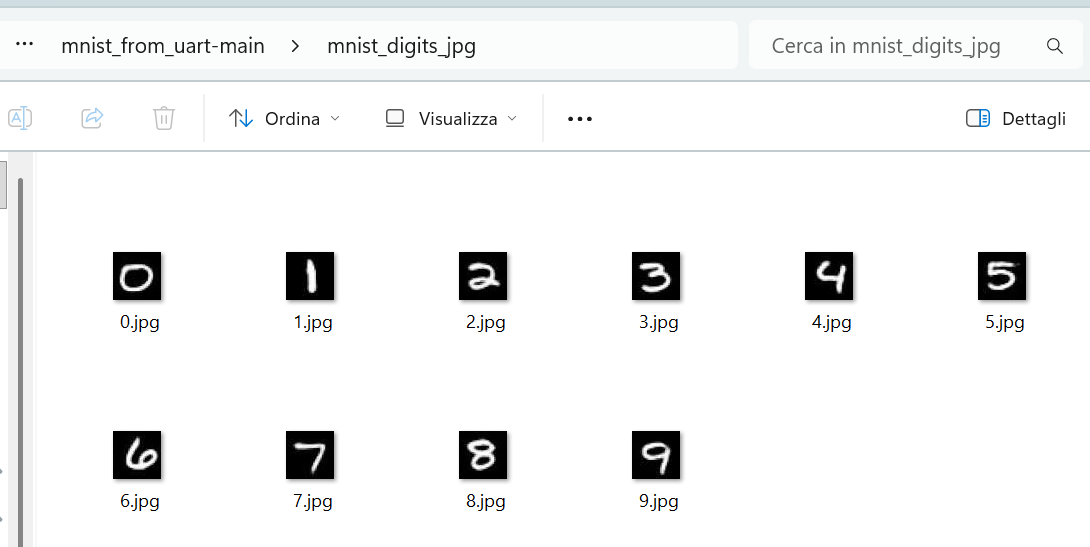
\includegraphics[width=0.85\textwidth]{images/test_image}
    \caption{Example of a MNIST handwritten digit image used as input for the DNN inference.}
    \label{fig:mnist}
\end{figure}

The flattened input vector is processed by a sequence of fully connected layers
with decreasing dimensionality, followed by non-linear activation functions.
Specifically, the baseline network consists of the following stages:
\begin{itemize}
    \item a fully connected layer mapping 784 input features to 64 neurons,
    \item a fully connected layer mapping 64 features to 32 neurons,
    \item a final fully connected layer mapping 32 features to 10 output classes.
\end{itemize}

Each intermediate fully connected layer is followed by a ReLU activation
function, while the output layer produces a vector of 10 scores corresponding to
the digit classes from 0 to 9.
This output vector is subsequently processed by a simple classification stage
that selects the class associated with the maximum score.

The baseline architecture represents a compact and regular reference model for
MNIST classification.
Its fully connected structure results in predictable memory access patterns and
a deterministic execution flow, making it well suited for implementation on
embedded processors without specialized hardware acceleration.

Figure~\ref{fig:onnx_base} shows the baseline DNN topology as visualized using
Netron.

\begin{figure}[H]
    \centering
    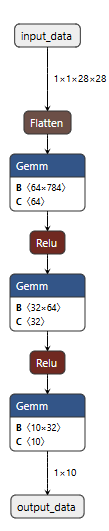
\includegraphics[width=0.25\textwidth]{images/onnx_model}
    \caption{Baseline MNIST DNN topology visualized using Netron.}
    \label{fig:onnx_base}
\end{figure}

The simplicity of the baseline network allows a direct one-to-one mapping between
the graphical representation provided by Netron and the corresponding C
implementation.
Each fully connected layer is explicitly implemented as a pair of nested loops
performing multiply--accumulate operations, while activation functions are
implemented as separate processing stages.
This clear separation of stages facilitates debugging, profiling, and further
optimization.

\section{Custom Network Topology (Group 4)}

In addition to the baseline network, a custom DNN topology was implemented
according to the group-specific assignment (Group~4).
The custom network extends the baseline architecture by introducing an additional
hidden fully connected layer, thereby increasing the depth of the network and the
overall computational workload.

The custom topology is composed of the following layers:
\begin{itemize}
    \item a fully connected layer mapping 784 input features to 64 neurons,
    \item a fully connected layer mapping 64 features to 32 neurons,
    \item a fully connected layer mapping 32 features to 16 neurons,
    \item a final fully connected layer mapping 16 features to 10 output classes.
\end{itemize}

As in the baseline case, ReLU activation functions are applied after each
intermediate layer, while the output layer produces a vector of class scores.
The introduction of an additional hidden layer increases both the number of
trainable parameters and the number of arithmetic operations required for a
single inference.

Figure~\ref{fig:onnx_group4} illustrates the custom DNN topology as visualized
using Netron.

\begin{figure}[H]
    \centering
    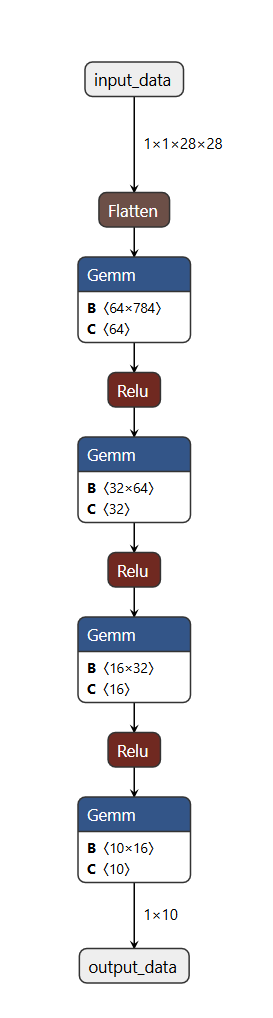
\includegraphics[width=0.22\textwidth]{images/onnx_model_group_4}
    \caption{Custom DNN topology for Group 4 visualized using Netron.}
    \label{fig:onnx_group4}
\end{figure}

The comparison between the baseline and the custom network provides a meaningful
case study for evaluating the scalability of the proposed software framework.
By increasing network depth while preserving the same implementation structure,
it is possible to analyze how architectural changes affect execution time,
memory usage, and real-time capability on the embedded platform.
Importantly, this scalability is achieved without requiring substantial
modifications to the overall software design, confirming the modularity and
extensibility of the implemented DNN inference pipeline.

\chapter{Fixed-Point DNN Implementation}

The Deep Neural Network inference is implemented entirely using fixed-point
arithmetic.
All weights, biases, inputs, and intermediate activations are represented using
16-bit signed integers (\texttt{int16}), enabling the elimination of floating-point
operations on the ARM Cortex-A9 processor.

This design choice is particularly suitable for embedded systems, where
floating-point units may introduce additional latency, non-deterministic execution
times, and higher energy consumption.
By relying exclusively on integer arithmetic, the implemented inference pipeline
achieves deterministic execution behavior and explicit control over numerical
precision, scaling, and overflow.

Figure~\ref{fig:fixed_point_math} illustrates the fixed-point accumulation strategy
adopted in the fully connected layers.


\begin{figure}[H]
\centering
\begin{tikzpicture}[
    scale=0.75,
    transform shape,
    node distance=10mm,
    every node/.style={
        draw,
        rounded corners,
        align=center,
        minimum width=42mm,
        minimum height=8mm
    },
    arrow/.style={->, thick}
]


% Nodes
\node (input) {Input vector $x_i$\\\small int16 -- Q-format};

\node (weight) [below=of input]
{Weights $w_i$\\\small int16 -- Q-format};

\node (mul) [below=of weight]
{Multiply\\\small $x_i \cdot w_i$};

\node (acc) [below=of mul, minimum height=12mm]
{64-bit Accumulator\\\small $\sum (x_i \cdot w_i)$};

\node (bias) [right=18mm of acc]
{Bias addition\\\small $(\text{bias} \ll QF)$};

\node (shift) [below=of acc]
{Right shift\\\small $\gg QF$};

\node (out) [below=of shift]
{Output neuron\\\small int16 -- Q-format};

% Arrows
\draw[arrow] (input) -- (weight);
\draw[arrow] (weight) -- (mul);
\draw[arrow] (mul) -- (acc);
\draw[arrow] (bias) -- (acc);
\draw[arrow] (acc) -- (shift);
\draw[arrow] (shift) -- (out);

\end{tikzpicture}
\caption{Conceptual fixed-point multiply--accumulate (MAC) operation used in the
fully connected layers. Inputs and weights are multiplied using fixed-point
arithmetic, accumulated with extended 64-bit precision, and scaled back to a
16-bit output representation through an explicit right-shift operation.}
\label{fig:fixed_point_math}
\end{figure}




\section{Data Representation and Q-Format}

All real-valued quantities in the DNN are encoded using a Q-format fixed-point
representation.
In the baseline configuration, network parameters and activations are represented
using a Q8.8 format, where 8 bits are allocated to the integer part and 8 bits to
the fractional part.

The Q8.8 format provides a good trade-off between numerical precision and dynamic
range for MNIST classification, while remaining fully compatible with 16-bit
integer arithmetic.
This representation is used as the reference configuration for functional
validation and performance comparison.

In addition to the baseline format, alternative fixed-point configurations are
supported through compile-time selection.
In particular, the optimized configuration (Tip~2) adopts a Q1.7 format for
weights and biases, increasing the available dynamic range while preserving
sufficient fractional precision.
The selected Q-format is controlled by the compile-time constant \texttt{QF},
ensuring deterministic behavior and reproducible measurements across different
runs.

Operationally, the Q-format is implemented by scaling real-valued quantities by
a factor of $2^{\texttt{QF}}$ prior to quantization, and by applying a symmetric
right shift after accumulation to restore the target fixed-point representation.
The offline conversion process used to generate Q1.7 parameters from the original
Q8.8 representation is described in Appendix~\ref{sec:appendix_tip2}.



\section{Multiply--Accumulate Operations}

Each fully connected layer is implemented explicitly as a sequence of
multiply--accumulate (MAC) operations.
For each output neuron, the dot product between the input vector and the
corresponding weight vector is computed.

To preserve numerical accuracy and avoid intermediate overflow, accumulation is
performed using a 64-bit signed integer accumulator.
Bias terms are added at the beginning of the accumulation process and are aligned
according to the selected Q-format, ensuring that bias contribution is accumulated
with the same numerical precision as the weighted sum.
After completion of the accumulation, the result is scaled back to the target
fixed-point representation by means of a right-shift operation proportional to
the fractional length.
The right-shift operation corresponds to a division by $2^{\texttt{QF}}$ and
restores the fixed-point scaling expected by subsequent layers.

This implementation directly reflects the arithmetic structure of the DNN and
allows fine-grained control over scaling and precision at each layer.
The adopted fixed-point MAC strategy is conceptually illustrated in
Figure~\ref{fig:fixed_point_math}.


\section{Saturation and Overflow Control}

To ensure predictable behavior in an embedded execution context, the
implementation explicitly considers saturation and overflow control.
Potential overflow conditions may arise during the accumulation phase of the
multiply--accumulate operations, where partial sums grow proportionally to the
number of input features and weight magnitudes.
A saturation function is provided to clamp accumulated values exceeding the
representable range of a 16-bit signed integer.

In the tested configurations (Q8.8 and Q1.7), no overflow conditions were observed
during experimental validation across all evaluated inputs and network layers.
For this reason, saturation is not actively applied in the main inference loop in
order to avoid unnecessary overhead and conditional branches that could negatively
impact execution time predictability.
However, the saturation mechanism is intentionally retained in the codebase to
support future extensions, such as reduced-precision implementations or more
aggressive scaling strategies.

This design choice balances robustness and performance, preserving deterministic
execution while maintaining extensibility for future architectural or numerical
modifications.


\section{Activation Functions}

Non-linear activation functions are implemented explicitly using integer
arithmetic.
In particular, the Rectified Linear Unit (ReLU) function is applied after each
intermediate fully connected layer.
The ReLU function is particularly well suited for fixed-point implementations,
as it does not require multiplications, divisions, or rescaling operations.

The ReLU operation is implemented as a simple comparison followed by a conditional
assignment that sets negative values to zero.
This implementation is computationally inexpensive and introduces negligible
overhead compared to the fully connected layers, where the dominant
multiply--accumulate workload is concentrated.
As a result, the execution time of the activation stage is data-independent and
fully deterministic, which is a desirable property in real-time embedded systems.


\section{Compile-Time Configurability}

All fixed-point configurations are selected at compile time using preprocessor
macros.
Configuration selection is implemented through preprocessor directives that
statically include the appropriate data representations and arithmetic paths
at compilation time.
This approach avoids runtime branching, ensures deterministic execution paths,
and enables fair performance comparison between different configurations.

Specifically, the implementation supports:
\begin{itemize}
    \item a baseline configuration with Q8.8 input data and parameters,
    \item an optimized configuration with compact Q0.8 input data (Tip~1),
    \item an extended optimized configuration with Q1.7 weights and biases
          (Tip~1 + Tip~2).
\end{itemize}

The compile-time selection mechanism guarantees that each configuration is
evaluated under identical execution conditions, excluding configuration-related
control flow from runtime execution and isolating the impact of data
representation choices on performance and robustness.


\section{Benefits of the Fixed-Point Design}

The fixed-point implementation provides several advantages in the context of
embedded systems:
\begin{itemize}
    \item complete elimination of floating-point operations and reliance on the FPU,
    \item reduced instruction count and computational overhead,
    \item deterministic execution times suitable for cycle-accurate profiling using
          the ARM Global Timer,
    \item explicit control over numerical precision, scaling, and overflow behavior,
    \item compatibility with communication-oriented optimizations and system-level
          profiling.
\end{itemize}

All these advantages are directly reflected in the experimental results presented
in the following chapters, where deterministic timing behavior and stable
cycle-level measurements are consistently observed.
These properties are fundamental for achieving reliable, efficient, and
predictable DNN inference on a general-purpose embedded processor, demonstrating
that fixed-point software-based implementations can meet real-time constraints
even in the absence of dedicated hardware accelerators.


\chapter{UART-Based DNN Microserver}

This chapter describes the communication architecture adopted to implement the
DNN microserver.
The microserver is responsible for receiving input data from an external host,
executing the neural network inference, and returning the classification result
to the host system.

An overview of the adopted UART-based microserver architecture is shown in
Figure~\ref{fig:uart_microserver_arch}.
The system follows a request--response microserver model, where the host
explicitly triggers inference by transmitting input samples, and the embedded
platform responds with the corresponding classification output.

Communication between the host PC and the embedded platform is implemented using
a UART-based interface.
This design choice reflects a realistic embedded scenario, where data are often
acquired through low-bandwidth serial links, and enables a direct comparison with
the communication models adopted in previous laboratory assignments, while
maintaining full control over data transfer timing and synchronization.


\begin{figure}[H]
\centering
\begin{tikzpicture}[
    font=\footnotesize,
    node distance=10mm,
    box/.style={
        draw,
        thick,
        rounded corners=2mm,
        minimum width=38mm,
        minimum height=10mm,
        align=center,
        fill=gray!5
    },
    arrow/.style={
        ->,
        thick
    }
]

% ================= HOST =================
\node[box, fill=blue!8] (host) {%
    \textbf{Host PC}\\
    Python Client\\
    (Image Streaming)
};

% ================= UART =================
\node[box, right=18mm of host, fill=gray!15] (uart) {%
    \textbf{UART Interface}\\
    Serial Link
};

% ================= EMBEDDED =================
\node[box, right=18mm of uart, fill=green!8] (ps) {%
    \textbf{Zybo Z7 -- PS}\\
    ARM Cortex-A9
};

% ================= DNN =================
\node[box, below=10mm of ps, fill=orange!10] (dnn) {%
    \textbf{DNN Inference Engine}\\
    Fixed-Point (Q-format)
};

% ================= TIMER =================
\node[box, below=10mm of dnn, fill=red!8] (timer) {%
    \textbf{Global Timer}\\
    Cycle Measurement
};

% ================= OUTPUT =================
\node[box, below=10mm of host, fill=purple!8] (out) {%
    \textbf{Classification Output}\\
    Predicted Digit
};

% ================= ARROWS =================
\draw[arrow] (host) -- node[above]{Input data} (uart);
\draw[arrow] (uart) -- node[above]{UART RX} (ps);
\draw[arrow] (ps) -- (dnn);
\draw[arrow] (dnn) -- (timer);
\draw[arrow] (dnn.west) |- (uart.south);
\draw[arrow] (uart.south) |- (out.east);

\end{tikzpicture}
\caption{UART-based DNN microserver architecture. The host PC streams input data to
the embedded platform, which performs fixed-point inference and returns the
classification result over the same serial interface.}
\label{fig:uart_microserver_arch}
\end{figure}


\section{Input Streaming Architecture}

MNIST images are streamed from a host PC to the Zybo Z7 board via UART as raw pixel
values.
Each image consists of 784 samples corresponding to a grayscale image of size
$28 \times 28$ pixels.

Data reception is implemented using a blocking strategy, where the application
waits until the complete image has been received before starting the inference
process.
At implementation level, this behavior is realized through a blocking UART
receive loop that explicitly waits for all 784 pixel values before enabling
the inference stage.

This approach simplifies synchronization between communication and computation
and ensures a clear separation between input acquisition and neural network
execution.

Each pixel is transmitted as a fixed-point value and reconstructed on the
embedded platform according to the active fixed-point configuration.
This design allows seamless integration with the fixed-point inference pipeline
described in the previous chapter and avoids any implicit data conversion during
runtime.

In the baseline configuration, each pixel is transmitted using two bytes,
corresponding to a Q8.8 fixed-point representation.
While straightforward, this approach introduces significant communication
latency due to the limited UART bandwidth.


Figure~\ref{fig:lab5_predicted_base} shows an example of the UART-based streaming
process for a single MNIST image, including raw data reception, inference
execution, and classification result transmission during the validation phase.


\begin{figure}[H]
    \centering
    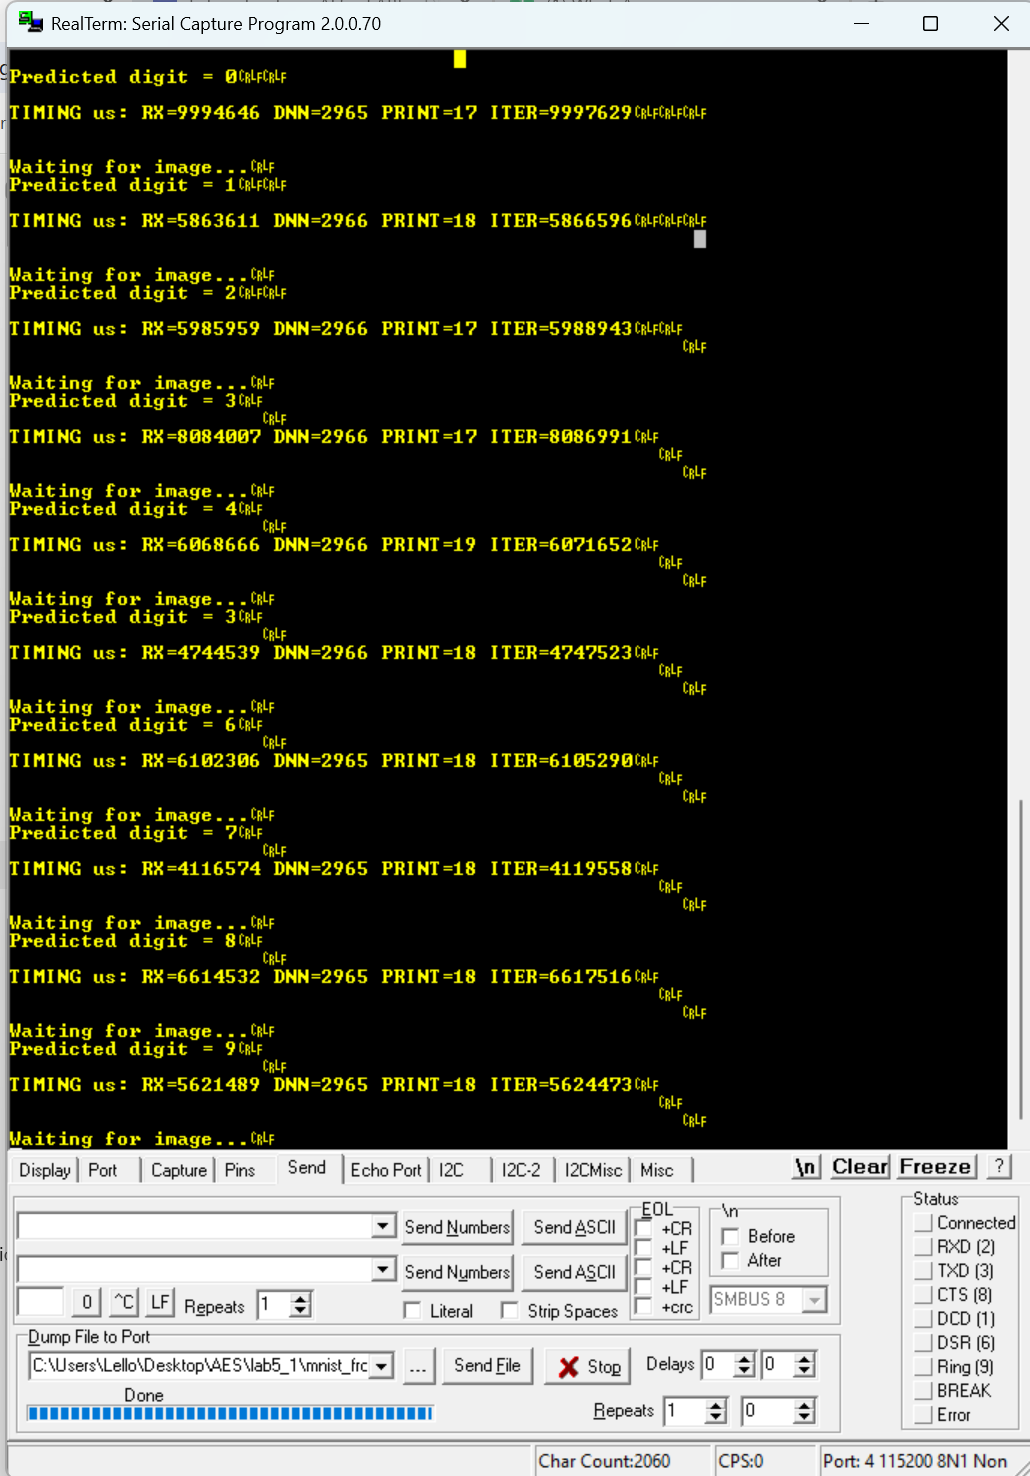
\includegraphics[width=0.65 \textwidth]{images/lab5_predicted_base}
  \caption{UART-based streaming and inference for a MNIST image during
    functional validation, showing input reception, predicted class, and serial
    output.}
    \label{fig:lab5_predicted_base}
\end{figure}


To address this limitation, an optimized input streaming mode (Tip~1) is
implemented.
In this configuration, each pixel is transmitted using a compact Q0.8
representation, encoded in a single byte.
On the embedded platform, pixel values are reconstructed into the internal
fixed-point format before being processed by the DNN.
This reconstruction is performed through a deterministic bit-shift operation,
ensuring correct alignment with the internal Q-format used by the inference
engine.

This optimization effectively halves the amount of data transferred over UART,
significantly reducing input reception time without affecting inference
correctness.
The offline preprocessing procedure used to generate Q0.8 input images is
described in Appendix~\ref{sec:appendix_tip1}.
The selection between baseline and optimized input streaming modes is performed
at compile time, guaranteeing deterministic behavior and enabling fair
performance comparison.

\section{Blocking Reception and Deterministic Behavior}

UART reception is implemented using a blocking byte-level read function.
The application explicitly waits until each expected byte is received, ensuring
that the full input image is available before inference begins.
At code level, this is implemented through a blocking polling loop on the UART
receive register, ensuring that no partial or incomplete image is ever processed.

Although blocking I/O is not optimal for high-throughput systems, it is
deliberately adopted in this laboratory activity to:
\begin{itemize}
    \item simplify control flow and synchronization,
    \item guarantee deterministic execution order,
    \item enable precise separation of communication and computation timing.
\end{itemize}

This design choice aligns with the educational objectives of Advanced Embedded
Systems and allows direct comparison with the timing methodologies introduced in
Laboratories~3 and~4.
As a result, both communication latency and computation time can be measured
independently and reproducibly, providing a deterministic execution model
suitable for fine-grained performance profiling.


\section{Functional Validation Using Embedded Test Images}

Before enabling real-time UART-based streaming, the correctness of the DNN
implementation is validated using statically linked MNIST test images.
This validation phase is critical to decouple functional verification of the
neural network from potential communication-related issues.

A set of reference MNIST images, corresponding to digits from 0 to 9, is embedded
directly into the application as header files.
Each image is processed by the DNN inference pipeline, and the predicted digit is
compared against the expected label.
At implementation level, these reference images are included as static arrays
and processed using the same inference functions adopted during online
UART-based execution.

This offline validation is performed entirely without UART communication and
therefore reflects pure computational correctness.
This offline validation step confirms:

\begin{itemize}
    \item correctness of the network topology and parameter loading,
    \item correctness of the fixed-point arithmetic implementation,
    \item correct operation of activation functions and result processing.
\end{itemize}

Only after successful validation of all embedded test images is the system
switched to UART-based online inference.
This staged validation approach significantly simplifies debugging and ensures
that any observed performance or classification issues during online execution
can be attributed to communication effects rather than to errors in the neural
network implementation.

Figure~\ref{fig:static_test} shows an example of the serial output produced during
the functional validation phase.

\begin{figure}[H]
    \centering
    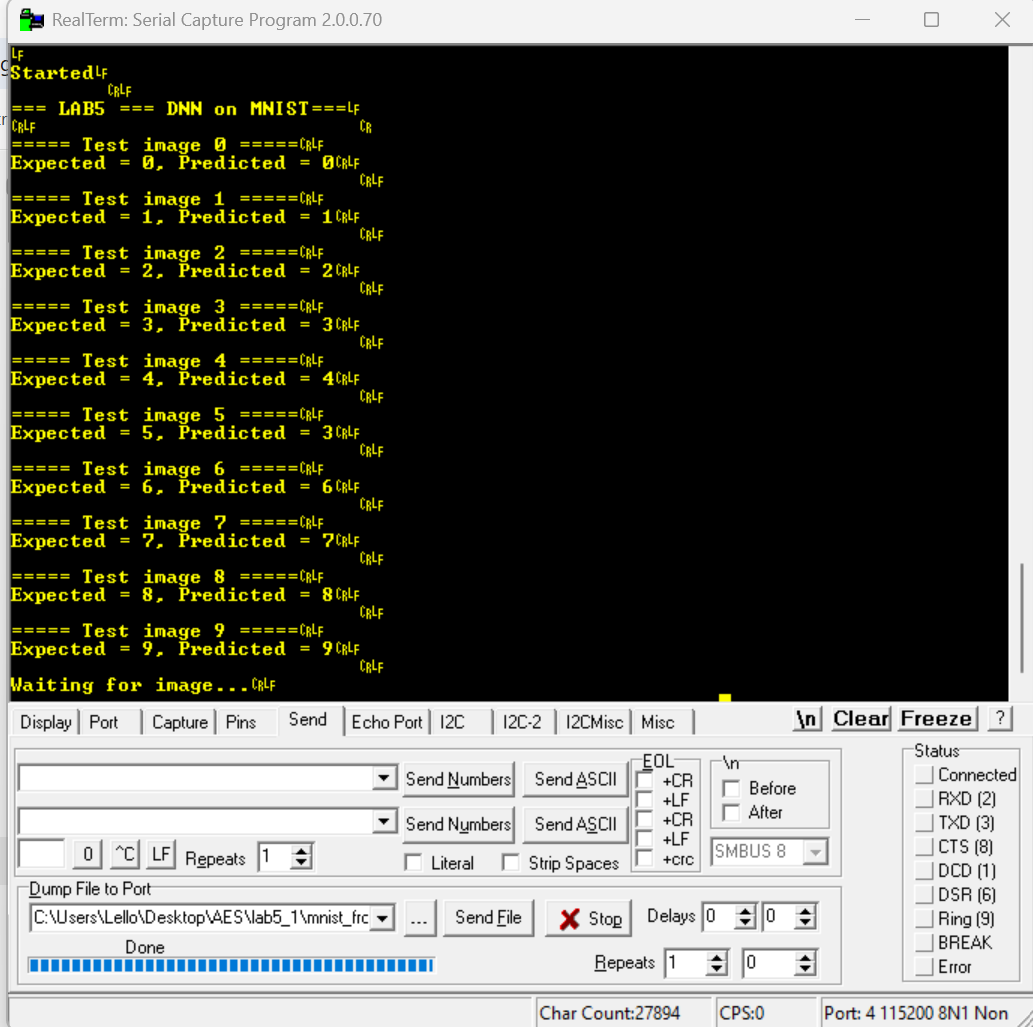
\includegraphics[width=1\textwidth]{images/lab5_start_test}
    \caption{Functional validation using statically linked MNIST test images.}
    \label{fig:static_test}
\end{figure}

The offline consistency checks between embedded test images and binary images
used for UART streaming are described in Appendix~\ref{sec:appendix_validation}.


\chapter{Execution Time Measurement}

Accurate execution time measurement is a fundamental aspect when evaluating the
feasibility of Deep Neural Network inference on embedded platforms.
In this work, timing measurements are performed using the 64-bit ARM Global Timer
available in the Processing System of the Zynq-7000 SoC, enabling fine-grained and
deterministic profiling of the entire inference pipeline.
This approach extends the timing methodologies adopted in previous laboratories
to a complete application-level workload that includes both communication and
computation stages.

The Global Timer provides a hardware-based timing source that is independent of
software overhead and operating system interference.
This makes it particularly suitable for performance analysis in standalone
embedded applications, where reproducibility and deterministic behavior are
required.
The use of a dedicated hardware timer ensures that measured execution times are
not affected by software jitter, background activities, or instrumentation
overhead.


\section{Measurement Methodology}

Execution time measurements are obtained using the ARM Cortex-A9 Global Timer
through the \texttt{XTime\_GetTime()} API.
The Global Timer implements a free-running 64-bit counter incremented at a fixed
frequency, allowing direct measurement of elapsed clock cycles with minimal
instrumentation overhead.

In the implemented code, timing is performed by reading the Global Timer counter
at multiple points within the main inference loop.
At implementation level, timing points are explicitly placed before and after
well-defined code sections, without introducing additional control flow or
runtime dependencies.
The difference between two consecutive readings directly represents the number of
elapsed clock cycles for the corresponding code section.
Cycle counts are subsequently converted to time values using the known timer
frequency, enabling reporting in microseconds.
This conversion is performed using the nominal Global Timer frequency provided
by the Zynq-7000 Processing System, ensuring consistent and reproducible timing
results.


Unlike previous laboratories, where execution time was measured by placing a
single start--end timer around a standalone computational kernel (e.g., vector
addition or FIR filtering), the objective of this laboratory is to characterize
the performance of a complete embedded inference pipeline.
As a result, timing instrumentation is distributed across different stages of
the application.

Specifically, the following stages are measured independently:
\begin{itemize}
    \item UART-based image reception time, measured by placing timer reads before
          and after the blocking reception loop;
    \item DNN inference time, including all fully connected layers and activation
          functions;
    \item result processing and output overhead, including classification and
          serial printing;
    \item total iteration time, measured by enclosing the complete inference
          cycle within a single timing window.
\end{itemize}

This multi-point measurement strategy enables a clear separation between
communication-bound and computation-bound components of the system, which is
essential for correct interpretation of performance results.
By instrumenting the application at multiple granularity levels, the adopted
methodology enables precise identification of dominant performance bottlenecks
and supports measurement-driven optimization.

The \texttt{XTime\_GetTime()} API provides access to the ARM Cortex-A9 Global Timer,
a 64-bit free-running hardware counter integrated in the Zynq-7000 Processing
System.
The timer is incremented at a fixed frequency and operates independently of the
processor execution flow and software activity.
As a result, timing measurements obtained through this interface accurately
reflect elapsed clock cycles and are not affected by operating system behavior,
software jitter, or peripheral interrupts.

\section{Warm-Up and Steady-State Measurements}

To ensure that the reported measurements reflect steady-state execution behavior,
the first iteration of the inference loop is intentionally discarded.
This warm-up iteration allows instruction caches, data caches, and branch
predictors to reach a stable state, avoiding artificially inflated timing results
caused by cold-start effects.
A single warm-up iteration is sufficient in this context, as the execution flow,
memory access patterns, and control paths remain invariant across subsequent
iterations.

All subsequent measurements are therefore representative of the deterministic
execution conditions encountered during continuous real-time operation of the
DNN microserver.

This approach is consistent with the methodology adopted in previous laboratories
and ensures fair comparison between baseline and optimized configurations.
By excluding the warm-up iteration, the collected measurements accurately
characterize steady-state performance and support reproducible, cycle-accurate
profiling of the inference pipeline.


\section{Separation of Communication and Computation}

A key aspect of the adopted timing methodology is the explicit separation between
communication time and computation time.
UART reception latency is dominated by serial bandwidth and host-side transmission
constraints, while DNN inference time reflects the actual computational workload
executed on the ARM Cortex-A9 processor.

At implementation level, this separation is achieved by placing independent
timing windows around the UART reception loop and the inference execution code.
By measuring these components independently, it is possible to:
\begin{itemize}
    \item identify the dominant performance bottleneck of the system,
    \item evaluate the impact of communication-oriented optimizations (e.g., Tip~1),
    \item assess the scalability of the inference pipeline independently of I/O
          constraints.
\end{itemize}

This separation is essential to correctly interpret the measured execution times
and to avoid conflating communication delays with computational inefficiencies.
In particular, this methodology allows overall system performance to be
interpreted in terms of communication-bound versus computation-bound behavior.


\section{Consistency with Previous Laboratories}

The timing strategy adopted in this laboratory represents a natural extension of
the methodologies introduced in Laboratories~3 and~4.
While earlier labs focused on cycle-accurate measurement of isolated kernels,
this work extends the same principles to a complete application-level workload.
In particular, the focus shifts from isolated computational kernels to an
integrated system that includes communication, control flow, and inference
execution.

The use of the ARM Global Timer across all laboratories ensures methodological
consistency and allows meaningful comparison between different types of embedded
workloads, ranging from signal processing to neural network inference.

Overall, the adopted measurement methodology provides a reliable and reproducible
characterization of execution time, forming the basis for the performance
evaluation and optimization analysis presented in the following chapters.
This methodological continuity ensures that the performance results discussed
in the following chapters can be interpreted in a coherent and comparable
framework.


\section{Per-Layer Profiling}

Each stage of the inference pipeline is profiled independently using the ARM
Global Timer.
In particular, execution time is measured for each fully connected layer and
for the associated activation functions.
At implementation level, this is achieved by placing dedicated timing windows
around each fully connected layer and its corresponding activation stage.

This per-layer profiling approach allows precise identification of the most
computationally intensive stages of the network and provides direct insight into
how network depth and layer dimensions affect overall performance.
This analysis is particularly relevant when comparing the baseline network with
the deeper custom topology adopted by Group~4.

By instrumenting the code at multiple points, it is possible to isolate the cost
of individual layers rather than relying on a single aggregate measurement.

Experimental results clearly show that the fully connected layers dominate the
computational cost of inference.
This behavior is expected for dense neural networks, where the bulk of the
execution time is spent performing multiply--accumulate operations.
In contrast, activation functions such as ReLU contribute only a negligible
fraction of the total inference time, due to their simple comparison-based
implementation.

Although the laboratory template includes a softmax computation during the result
processing stage, the final classification decision is effectively determined by
an argmax operation on the output logits.
As a consequence, the softmax computation does not influence the predicted class
and is not performance-critical in the current implementation.
For this reason, its impact on overall execution time is negligible compared to
that of the fully connected layers.

Figure~\ref{fig:timing} shows a representative execution time breakdown obtained
during real-time inference, highlighting the relative contribution of each
processing stage.

\begin{figure}[H]
    \centering
    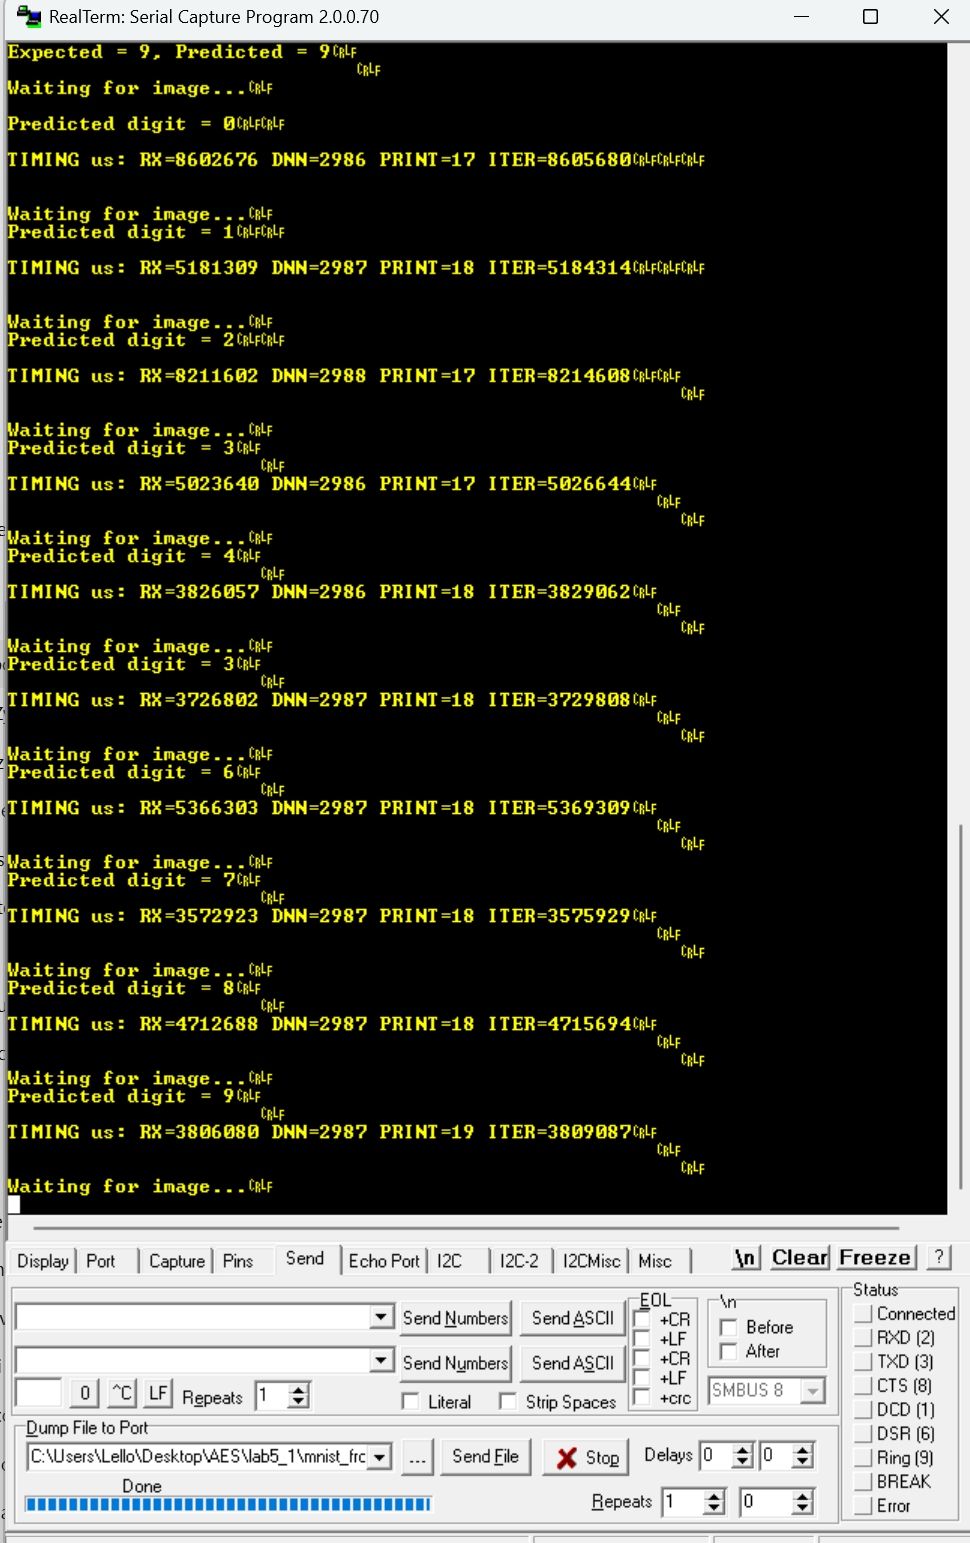
\includegraphics[width=1\textwidth]{images/lab5_start_test_Custom_UART}
    \caption{Per-layer execution time breakdown measured using the ARM Global Timer.}
    \label{fig:timing}
\end{figure}

\section{Communication Versus Computation}

The explicit separation between communication time and computation time is a key
aspect of the adopted performance analysis.
In the context of an embedded DNN microserver, overall system performance depends
not only on the efficiency of the inference algorithm, but also on the latency of
the communication interface used to acquire input data.

Experimental measurements show that the time required to receive a complete MNIST
image via UART is orders of magnitude larger than the time required to execute the
DNN inference itself.
While inference requires only a few milliseconds per image, UART-based reception
may require several seconds, depending on transmission parameters and host-side
behavior.

This result demonstrates that, under the considered configuration, the system is
compute-efficient and that overall throughput is primarily limited by
communication bandwidth rather than by processing capability.
In other words, the application operates in a communication-bound regime, where
optimizations targeting data transfer have a much greater impact on system
performance than further computational acceleration.

Such an analysis provides a solid basis for evaluating communication-oriented
optimizations, such as compact input data representation (Tip~1), and for
assessing the real-time feasibility of the proposed microserver architecture.
By clearly distinguishing between communication and computation costs, the
adopted methodology enables informed design decisions and avoids misleading
performance interpretations.
ntitative evaluation of software
optimizations and architectural design choices.




\chapter{Optimization Tips and Custom Enhancements}

In addition to the baseline implementation, several optimization strategies were
explored by modifying the representation of input data and network parameters, as
suggested in the laboratory guidelines.
The objective of these enhancements is not to alter the functional behavior of the
DNN inference pipeline, but to improve system-level efficiency, numerical robustness,
and configurability under embedded constraints.

All optimizations are implemented in a configurable and modular manner, enabling
direct comparison between baseline and optimized configurations through compile-time
selection, without modifying the overall software architecture or control flow.

\section{Input Data Optimization}

In the baseline configuration, input images are transmitted via UART using a Q8.8
fixed-point representation, where each pixel is encoded using two bytes.
While this format simplifies direct integration with the internal fixed-point
pipeline, it introduces a significant communication overhead on a low-bandwidth
serial interface.

As an optimization, input images are alternatively transmitted using a more compact
Q0.8 representation, where each pixel is encoded using a single byte.
On the embedded platform, pixel values are reconstructed into the internal
fixed-point representation before being processed by the DNN.

This optimization effectively reduces the amount of data transferred over UART by
approximately 50\%, leading to a proportional reduction in image reception time.
Experimental measurements confirm that this optimization primarily affects
communication latency, while leaving the computational behavior of the inference
pipeline unchanged.

From a system-level perspective, this approach directly targets the dominant
bottleneck identified in the baseline analysis, namely UART-based data transfer,
and therefore represents a communication-oriented optimization rather than a
computational one.

\section{Weight and Bias Representation}

A second optimization concerns the representation of network weights and biases.
In the baseline configuration, all parameters are encoded using a Q8.8 fixed-point
format.
While sufficient for MNIST classification, this format may limit dynamic range and
increase the risk of saturation effects in deeper network configurations.

To address this issue, an alternative Q1.7 representation is adopted for weights and
biases.
By allocating an additional bit to the integer part, this format increases dynamic
range while preserving fractional precision compatible with 16-bit fixed-point
arithmetic.

In the implemented system, the conversion from Q8.8 to Q1.7 is performed offline,
and parameters are stored directly in the optimized format.
As a result, no additional runtime overhead is introduced, and deterministic
execution behavior is preserved.

Experimental validation confirms that the use of Q1.7 weights and biases improves
numerical robustness and reduces the likelihood of saturation during accumulation,
particularly in the custom Group~4 network topology, without affecting functional
correctness.

\section{Configurability and Scalability}

All optimization options are controlled through compile-time configuration flags.
This design choice allows rapid switching between baseline and optimized operating
modes, facilitating systematic experimental evaluation and reproducibility of
performance results.

The same software framework supports both the baseline and custom DNN topologies,
demonstrating the scalability and modularity of the implementation.
Network depth, layer dimensions, and fixed-point formats can be modified without
affecting the overall structure of the code, highlighting the generality of the
adopted design.

\section{Impact on Performance}

Experimental results show that the explored optimizations do not compromise the
functional correctness of the DNN inference.
Instead, they provide tangible benefits in terms of reduced communication overhead
and improved numerical stability.

In particular, input data optimization directly reduces UART reception time, while
the alternative representation of weights and biases enhances robustness in deeper
network configurations.
These results confirm that careful data representation choices and system-level
design decisions play a crucial role in achieving efficient and scalable embedded
AI implementations, even in the absence of hardware acceleration.


\chapter{Validation and Debugging of Input Data Consistency}

During functional validation of the baseline and custom DNN architectures,
an anomalous classification behavior was observed for a specific input class.
In particular, both the baseline network and the custom Group~4 topology
systematically failed to correctly classify the handwritten digit ``5'',
while all other digits were recognized correctly.

This behavior was observed consistently across multiple executions and fixed-point
configurations, suggesting that the issue was not related to numerical instability,
quantization effects, or network topology, but rather to a potential inconsistency
in the input data representation.

Given that the same DNN parameters correctly classified the digit ``5'' when using
embedded test images, the source of the misclassification was hypothesized to lie
in the preprocessing or transmission pipeline of the MNIST images used for
UART-based inference.

In particular, possible causes included:
\begin{itemize}
    \item unintended scaling differences between embedded images and binary images;
    \item truncation effects introduced during fixed-point format conversion;
    \item endianness mismatches in binary file generation or parsing;
    \item inconsistencies between statically linked test images and externally
          streamed input data.
\end{itemize}

To systematically investigate these hypotheses, a dedicated offline validation
and debugging tool was developed to perform a pixel-wise consistency check between
embedded MNIST images and their corresponding binary representations.
The validation tool, implemented in Python and reported in
Appendix~\ref{sec:appendix_validation}, compares:
(i) MNIST images embedded in the C source code as static macros
(\texttt{test\_images.h, imm\_test\_X}), and
(ii) MNIST images stored as raw binary files (\texttt{.bin}) used for UART-based
inference testing.

The script automatically detects the fixed-point scale of the binary images
(Q8.8 or Q0.8), aligns representations, and computes pixel-wise differences.
Both numerical diagnostics and visual comparisons are produced to support
robust debugging and traceability.

\begin{figure}[H]
    \centering
    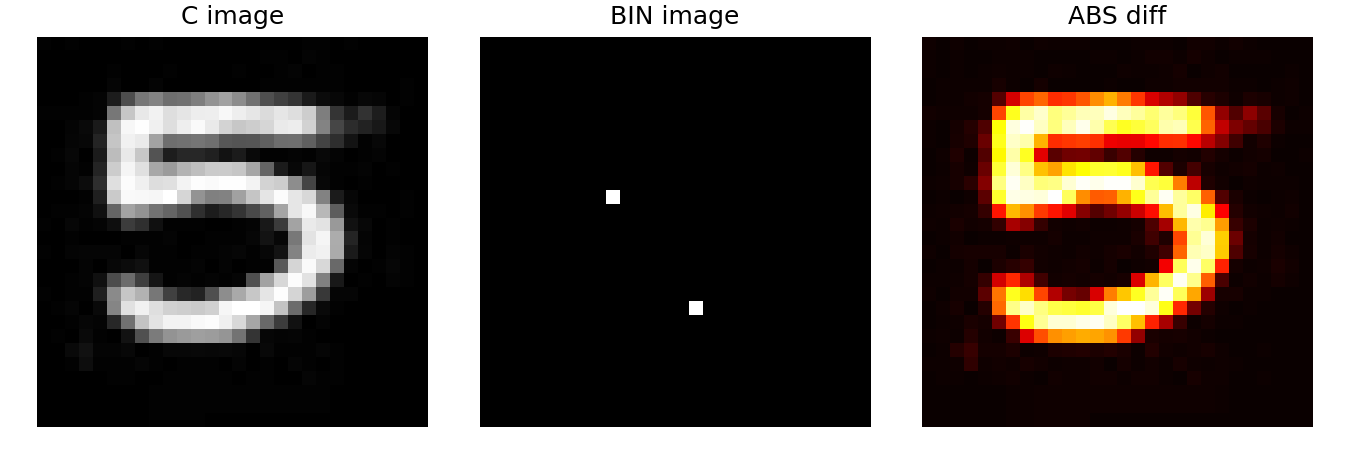
\includegraphics[width=0.95\textwidth]{images/digit_5_compare}
    \caption{Offline consistency check for digit ``5''. From left to right:
    embedded MNIST image (C macro), binary image used for UART-based inference,
    and absolute pixel-wise difference.
    The visualization highlights localized discrepancies responsible for
    systematic misclassification.}
    \label{fig:digit5_diff}
\end{figure}

The consistency analysis revealed that the digit ``5'' exhibited non-zero
pixel-wise differences between the embedded representation and the binary
image used for UART-based inference, whereas all other digits showed either
perfect or near-perfect correspondence.

As a consequence, the observed misclassification was attributed to input data
inconsistencies rather than to deficiencies in the DNN architecture, fixed-point
arithmetic, or inference pipeline.

This validation step proved essential to ensure experimental correctness and
demonstrates the importance of systematic data verification in embedded AI
applications, where preprocessing and communication stages may silently introduce
errors that are difficult to detect at runtime.


\chapter{Performance Evaluation}

This chapter presents a quantitative evaluation of the proposed UART-based DNN
microserver, focusing on execution time, communication latency, and overall
end-to-end performance.
All measurements are obtained on the Zybo Z7 platform using the methodology
described in Chapter~6 and are based on cycle-accurate timing derived from the ARM
Global Timer.

Performance is evaluated under three fixed-point configurations:
(i) a baseline configuration using Q8.8 input data and parameters,
(ii) an optimized configuration employing compact Q0.8 UART input streaming
(Tip~1),
and (iii) a combined optimized configuration using Q0.8 input data and reduced
Q1.7 weights and biases (Tip~1 + Tip~2).

For each configuration, execution time is decomposed into communication time,
inference time, and output overhead, enabling a detailed analysis of performance
bottlenecks and optimization effectiveness.
All reported measurements refer to steady-state execution conditions, with warm-up
iterations discarded as discussed in Chapter~6.

\begin{table}[H]
\centering
\caption{Average execution time breakdown under different fixed-point configurations}
\label{tab:perf_summary}
\renewcommand{\arraystretch}{1.2}
\begin{tabular}{|l|c|c|c|c|}
\hline
\textbf{Configuration} & \textbf{RX [µs]} & \textbf{DNN [µs]} & \textbf{PRINT [µs]} & \textbf{ITER [µs]} \\
\hline
Baseline (Q8.8) & 5\,064\,059 & 2\,988 & 18 & 5\,067\,065 \\
Tip~1 (Q0.8) & 3\,486\,914 & 2\,988 & 18 & 3\,489\,920 \\
Tip~1 + Tip~2 (Q1.7) & 3\,690\,949 & 2\,988 & 18 & 3\,693\,955 \\
\hline
\end{tabular}
\end{table}

Table~\ref{tab:perf_summary} summarizes the average execution time breakdown
measured under the different fixed-point configurations.

The experimental results clearly show that UART communication dominates the
overall execution time in all configurations.
In the baseline setup, more than 99\% of the end-to-end latency is attributable to
input reception, while DNN inference accounts for less than 0.1\% of the total
iteration time.

This highlights that the computational workload of the fixed-point DNN is
negligible compared to the cost of serial data transfer over UART.

The adoption of compact Q0.8 input streaming (Tip~1) significantly reduces UART
latency, achieving an average UART reception time reduction of approximately 31\% with
respect to the baseline configuration.

This improvement directly translates into a proportional reduction of the total
iteration time, confirming that the system is communication-bound.

In contrast, the use of reduced-precision Q1.7 weights and biases (Tip~2) does not
affect inference execution time, as the computational structure and number of
multiply--accumulate operations remain unchanged.



\section{Compute-Only Throughput}

To evaluate the intrinsic computational efficiency of the DNN implementation,
a compute-only throughput metric is adopted.
This metric is obtained by excluding the time required for UART-based data
reception and considering only the execution time of the neural network
inference itself.

By isolating computation from communication, it is possible to assess the
processing capabilities of the ARM Cortex-A9 independently of external I/O
constraints.
Compute-only throughput is expressed in terms of processed images per second
(img/s) and is computed as the inverse of the measured DNN inference time.

Experimental results show that the inference pipeline executes in approximately
a few milliseconds per image, corresponding to a throughput on the order of
several hundred images per second.
These values remain highly stable across repeated executions, confirming the
deterministic behavior of the fixed-point implementation and the absence of
data-dependent execution time variations.

This result demonstrates that the computational workload imposed by the
considered DNN topology is well within the processing capabilities of the target
embedded platform, leaving substantial computational headroom for potential
extensions such as deeper networks or additional processing stages.

\section{Real-Time Capability Analysis}

The real-time capability of the system is evaluated by comparing the execution
time of the DNN inference with the time required to acquire an input image via
UART.
Experimental measurements show that the inference time is orders of magnitude
smaller than the communication latency associated with serial data transfer.

As a consequence, each image is fully processed well within the time window
defined by the arrival of the next input sample.
The inference pipeline therefore does not introduce any backlog or data loss
when images are streamed sequentially from the host computer.

This observation confirms that the proposed implementation satisfies real-time
requirements under the considered operating conditions.
In particular, the system operates in a communication-bound regime, where
overall throughput is limited by UART bandwidth rather than by computational
performance.

Figure~\ref{fig:throughput} illustrates the measured throughput and clearly
highlights the separation between communication-dominated and
computation-dominated phases of the execution.

\begin{figure}[H]
    \centering
    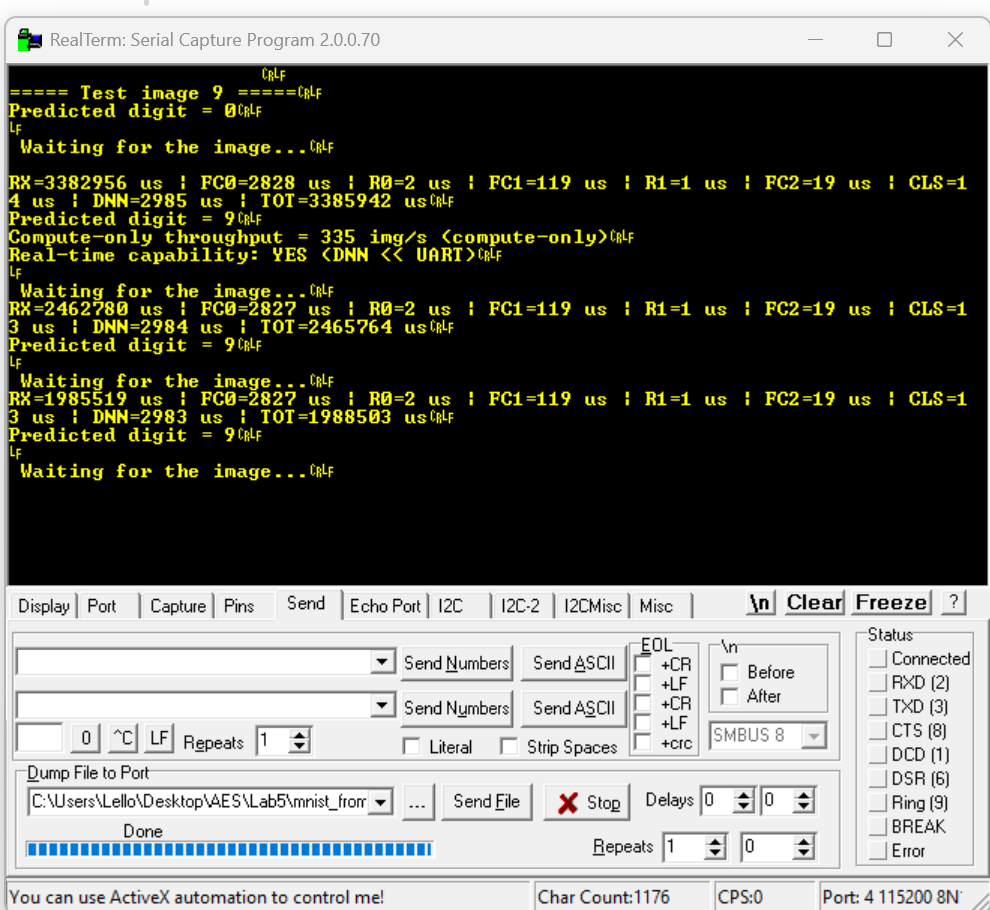
\includegraphics[width=1\textwidth]{images/lab5_Throughput.png}
    \caption{Measured compute-only throughput and real-time capability.}
    \label{fig:throughput}
\end{figure}


At the same time, it confirms that the adopted fixed-point DNN implementation is
efficient, predictable, and suitable for real-time embedded deployment.

\section{Baseline Performance Results}

These values were obtained from repeated executions of the real-time inference loop,
measured using the ARM Global Timer and collected through UART debug output.

Across multiple iterations, the measured inference time remained highly stable
(2.98–2.99\,ms), confirming deterministic behavior under steady-state conditions.
This stability is a direct consequence of the standalone execution model, the
exclusive use of fixed-point arithmetic, and the absence of operating system
interference.

Per-layer profiling highlights that the first fully connected layer (784→64)
dominates the computational cost, accounting for more than 94\% of the total
inference time.
This result is consistent with the expected workload distribution in dense neural
networks, where the largest matrix--vector multiplication typically represents the
primary computational bottleneck.

In contrast, UART-based image reception requires between 2.0 and 3.4 seconds per
image, depending on transmission conditions.
As a result, overall system performance in the baseline configuration is strongly
communication-bound, while the inference pipeline itself easily satisfies real-time
constraints.

Measured UART reception times are therefore approximately three orders of magnitude
larger than the corresponding inference time, resulting in a
communication-to-computation ratio on the order of $10^3$.
This clearly indicates that system throughput is limited by serial communication
bandwidth rather than by the computational performance of the DNN inference pipeline.

From a system-level perspective, these results demonstrate that the proposed
software-based implementation not only satisfies real-time requirements, but also
leaves significant computational headroom for more complex network topologies or
additional processing stages.

All results presented in this section refer to the baseline configuration, with
Q8.8 input data and Q8.8 weights and biases, and without communication-oriented
optimizations enabled.


\section{Performance Results with Optimization Tips Enabled}

This section presents the performance evaluation of the optimized configuration,
in which the laboratory optimization tips are enabled.
In particular, two enhancements are considered:
(i) compact input data transmission using a Q0.8 format, and
(ii) alternative fixed-point representation for weights and biases using Q1.7.

The objective of this evaluation is to quantify the impact of these optimizations
on communication latency, numerical robustness, and overall system behavior,
while preserving functional correctness and real-time capability.

\subsection{Compute Performance}

When the optimization tips are enabled, the internal structure of the DNN inference
pipeline remains unchanged.
As a consequence, the compute-only execution time of the network is expected to
remain comparable to that of the baseline configuration.

Experimental measurements confirm this expectation.
The execution time of the DNN inference remains approximately constant at around
3\,ms per image, corresponding to a compute-only throughput in the range of
330–340 images per second.
This result demonstrates that the adopted optimizations do not introduce additional
computational overhead and preserve the deterministic execution behavior observed
in the baseline case.

The stability of the measured inference time across multiple iterations further
confirms that the use of alternative Q-formats does not negatively affect timing
predictability or execution determinism.

\subsection{Impact on Communication Latency}

The primary performance benefit of the optimized configuration is observed at the
communication level.
By transmitting input images using a Q0.8 representation, each pixel is encoded
using a single byte instead of two, effectively reducing the amount of data sent
over UART by approximately 50\%.

As a result, the time required to receive a full MNIST image is significantly
reduced compared to the baseline configuration.
Although the system remains communication-bound, the reduced reception time
improves overall responsiveness and increases the maximum sustainable input rate.

This optimization directly targets the dominant bottleneck identified in the
baseline analysis, namely UART-based data transfer, and therefore represents a
system-level optimization rather than a purely computational one.

\subsection{Numerical Robustness and Stability}

The use of a Q1.7 fixed-point format for weights and biases increases the dynamic
range available during accumulation in fully connected layers.
This reduces the risk of saturation effects, particularly in deeper network
configurations such as the custom Group~4 topology.

Experimental validation confirms that classification accuracy and functional
correctness are preserved under the optimized configuration.
No instability or anomalous behavior was observed during extended execution,
demonstrating that the alternative fixed-point representation is fully compatible
with the implemented inference pipeline.

\subsection{Discussion on Optimized Configuration}

The performance evaluation with optimization tips enabled highlights an important
system-level insight.
While computational performance remains essentially unchanged, communication
efficiency and numerical robustness are significantly improved.

These results confirm that, in embedded DNN microserver applications, effective
optimization strategies often target data representation and communication
mechanisms rather than raw computational acceleration.
The optimized configuration therefore provides a more balanced and robust system
design, while fully satisfying real-time requirements.

\section{Overall Discussion}

The performance evaluation presented in this chapter highlights a clear separation
between computation and communication costs in the proposed DNN microserver.
In both the baseline and optimized configurations, the inference pipeline exhibits
deterministic execution times on the order of a few milliseconds per image,
confirming the suitability of the fixed-point software-based implementation for
real-time operation on an embedded ARM Cortex-A9 processor.

The baseline analysis demonstrates that computation is not the limiting factor,
as inference time is orders of magnitude smaller than UART communication latency.
This observation is further reinforced by the optimized configuration, in which
communication-oriented enhancements significantly reduce input reception time
without affecting computational performance.

The comparison between baseline and optimized results confirms that system-level
optimizations targeting data representation and communication bandwidth are more
effective than purely computational optimizations in this context.
At the same time, the adoption of alternative fixed-point formats improves numerical
robustness, particularly for deeper network topologies, without compromising timing
predictability or functional correctness.

Overall, the obtained results validate the design choices adopted in this work and
demonstrate that careful software design, combined with measurement-driven analysis,
enables efficient and scalable deployment of Deep Neural Network inference on
resource-constrained embedded platforms.


\chapter{Conclusions}

This work demonstrates that a fully software-based Deep Neural Network can achieve
real-time MNIST classification on an embedded ARM Cortex-A9 platform when fixed-point
arithmetic and careful system-level design are employed.

Starting from the analysis of the DNN architecture using ONNX models and the Netron
visualization tool, the inference pipeline was manually mapped onto an embedded
processing system.
This process emphasized explicit control over data representation, memory
organization, and execution flow, which are key aspects in the deployment of AI
workloads on resource-constrained platforms.

The adoption of fixed-point arithmetic enabled the complete elimination of
floating-point operations, ensuring deterministic execution behavior and reducing
computational overhead.
This design choice proved particularly effective in a standalone execution
environment, where predictable timing and low-level control are essential for
accurate performance evaluation.

The implementation of a UART-based DNN microserver enabled a realistic assessment
of inference under communication constraints.
Experimental results clearly showed that, in the considered configuration, the
execution time of the DNN inference is orders of magnitude smaller than the
communication latency associated with UART-based image streaming.
As a result, the system operates in a communication-bound regime, while the
inference pipeline itself fully satisfies real-time requirements.

Cycle-accurate execution time measurements performed using the ARM Global Timer
provided detailed insight into the contribution of each processing stage.
Per-layer profiling highlighted the dominance of fully connected layers in the
computational workload and confirmed the effectiveness of the adopted measurement
methodology and optimization strategies.

Additional enhancements, including compact input data representation and alternative
fixed-point formats for network parameters, further improved communication efficiency
and numerical robustness without requiring changes to the core inference algorithm.
The successful extension to a custom Group~4 network topology demonstrated the
scalability and modularity of the proposed software framework.

Overall, this laboratory activity illustrates how Deep Neural Network inference can
be effectively deployed on a general-purpose embedded processor through careful
software design and measurement-driven optimization.
The results highlight the importance of system-level analysis when integrating AI
techniques into embedded platforms and provide a solid foundation for further
exploration of hardware--software co-design solutions.


\chapter{Appendix – Preprocessing Tools and Optimization Scripts}
\label{chap:appendix}

This appendix collects the Python tools developed to support the optimization,
validation, and experimental evaluation of the DNN microserver implemented in
Laboratory~5.

The scripts presented in this appendix are not part of the embedded application
executed on the Zybo Z7 platform, but were used offline to:
(i) preprocess network parameters and input data,
(ii) enable communication-oriented and numerical optimizations,
and (iii) validate the correctness and consistency of the experimental setup.

All tools are designed to be deterministic, reproducible, and directly traceable
to the corresponding optimizations discussed in the main body of the report.

\begin{table}[H]
\centering
\caption{Offline preprocessing and validation tools used in Laboratory~5}
\label{tab:appendix_tools}
\renewcommand{\arraystretch}{1.2}
\begin{tabular}{|l|c|p{7cm}|}
\hline
\textbf{Script} & \textbf{Tip} & \textbf{Purpose} \\
\hline
\texttt{bin2weights.py} &
Tip~2 &
Conversion of DNN weights and biases from Q8.8 to Q1.7 fixed-point format for
memory footprint reduction and improved numerical robustness. \\
\hline
\texttt{tip1\_q88\_to\_q08.py} &
Tip~1 &
Compression of MNIST input images from Q8.8 to Q0.8 to reduce UART bandwidth
by approximately 50\%. \\
\hline
\texttt{images\_test\_bin.py} &
Validation &
Offline consistency check between embedded MNIST images and binary images used
for UART-based inference, ensuring numerical equivalence and correct preprocessing. \\
\hline
\end{tabular}
\end{table}


\section{Overview of the Optimization Workflow}
\label{sec:appendix_workflow}
The optimization workflow adopted in this work is composed of three main stages:

\begin{itemize}
    \item offline quantization of input images for UART transmission optimization (Tip~1);
    \item offline conversion of network weights and biases to alternative fixed-point
          representations (Tip~2);
    \item functional validation of the baseline and custom DNN architectures using
          reference MNIST images.
\end{itemize}

All preprocessing steps are executed on the host PC using Python, while the
embedded platform executes only the fixed-point inference pipeline.
This separation allows isolating communication and computation effects and
ensures deterministic behavior during runtime measurements.



\section{Input Image Quantization (TIP 1)}
\label{sec:appendix_tip1}

In the baseline configuration, MNIST input images are transmitted over UART using
a Q8.8 fixed-point representation, requiring two bytes per pixel.
While this format simplifies integration with the internal fixed-point inference
pipeline, it introduces a significant communication overhead.

Tip~1 addresses this limitation by adopting a compact Q0.8 representation for
input images, where each pixel is encoded using a single byte.
The conversion is performed offline using a Python script that exploits the
numerical characteristics of MNIST data.

Since MNIST pixel values are normalized in the range \([0, 1)\),
their Q8.8 fixed-point representation is expected to lie within the interval
\([0x0000, 0x00FF]\).

Under this assumption, the most significant byte is always zero and can be safely
discarded during transmission.
As a result, UART payload is reduced by approximately 50\% without loss of
numerical information.


\subsection{Python Script for Q8.8 to Q0.8 Conversion}
\label{sec:appendix_tip1_script}

Listing~\ref{lst:tip1_q08} reports the Python script used to convert MNIST test
images from Q8.8 to Q0.8 fixed-point format.

The script processes binary image files in a deterministic order, performs
defensive clipping to handle potential out-of-range values, and generates compact
binary payloads suitable for UART transmission.
All conversions are executed offline on the host PC, ensuring that no additional
runtime overhead is introduced on the embedded platform.

\begin{lstlisting}[
language=Python,
caption={Python script for offline conversion of MNIST images from Q8.8 to Q0.8 format (UART optimization – Tip~1).},
label={lst:tip1_q08},
basicstyle=\ttfamily\footnotesize,
keywordstyle=\color{blue},
commentstyle=\color{gray},
stringstyle=\color{teal},
showstringspaces=false,
breaklines=true,
frame=single
]
#!/usr/bin/env python3
# ================================================================
#  tip1_q88_to_q08.py
#
#  Lab 5 – DNN on MNIST (UART Microserver – Tip 1)
#  Course: Advanced Embedded Systems (AES)
#  Board: Zybo Z7 – Zynq-7000 (ARM Cortex-A9)
#
#  Description:
#  ---------------------------------------------------------------
#  Tip 1 – UART Bandwidth Optimization
#
#  This script converts MNIST test images stored in Q8.8 fixed-point
#  format into a compact Q0.8 representation.
#
#  Author: Lello Molinario
# ================================================================

import os

SRC_DIR = "../test/mnist_digits_bin"
DST_DIR = "../test/mnist_digits_q08"

os.makedirs(DST_DIR, exist_ok=True)

for fname in sorted(os.listdir(SRC_DIR)):
    if not fname.endswith(".bin"):
        continue

    src_path = os.path.join(SRC_DIR, fname)
    base, _ = os.path.splitext(fname)
    dst_path = os.path.join(DST_DIR, base + "_q08.bin")

    with open(src_path, "rb") as f:
        data = f.read()

    if len(data) % 2 != 0:
        raise ValueError(f"{fname}: invalid file size")

    q08 = bytearray()

    for i in range(0, len(data), 2):
        lsb = data[i]
        msb = data[i + 1]
        value = (msb << 8) | lsb

        if value > 0x00FF:
            value = 0x00FF

        q08.append(value & 0xFF)

    with open(dst_path, "wb") as f:
        f.write(q08)

    print(f"{fname}: {len(data)} bytes → {len(q08)} bytes")

print("Conversion completed successfully.")
\end{lstlisting}


\section{Weight and Bias Conversion (TIP 2)}
\label{sec:appendix_tip2}

Tip~2 focuses on improving numerical robustness and memory efficiency by adopting
an alternative fixed-point representation for network weights and biases.

While the baseline implementation uses a Q8.8 fixed-point format, all network
parameters are converted offline to a Q1.7 representation in the optimized
configuration.
The conversion is performed using a dedicated Python script that processes the
original binary parameter files generated from the ONNX model.

The adopted conversion strategy consists of:
\begin{itemize}
    \item arithmetic right shift by one bit to convert Q8.8 values into Q1.7;
    \item explicit saturation to the signed 8-bit range \([-128, 127]\) to prevent
          overflow and ensure predictable behavior.
\end{itemize}

All conversions are executed offline on the host PC.
The resulting parameters are embedded directly in the application as static
C macros, avoiding any runtime overhead and preserving deterministic execution
behavior on the ARM Cortex-A9 processor.

\subsection{Python Script for Weight and Bias Conversion}
\label{sec:appendix_tip2_script}

Listing~\ref{lst:bin2weights} reports the Python script used to convert binary
weight and bias files from the baseline Q8.8 fixed-point format to both Q8.8
and Q1.7 representations.

The script reads little-endian signed 16-bit values, generates C-compatible
macros for static initialization, and produces a single header file containing
both baseline and optimized parameters.
This approach enables straightforward comparison between configurations and
supports reproducibility of the experimental results.

\begin{lstlisting}[
language=Python,
caption={Python script for offline conversion of DNN weights and biases from Q8.8 to Q1.7 (Tip~2).},
label={lst:bin2weights},
basicstyle=\ttfamily\footnotesize,
keywordstyle=\color{blue},
commentstyle=\color{gray},
stringstyle=\color{teal},
showstringspaces=false,
breaklines=true,
frame=single
]
#!/usr/bin/env python3
# ================================================================
#  bin2weights.py
#
#  Lab 5 – DNN on MNIST (Custom Network – Group 4)
#  Course: Advanced Embedded Systems (AES)
#  Board: Zybo Z7 – Zynq-7000 (ARM Cortex-A9)
#
#  Description:
#  ---------------------------------------------------------------
#  This script converts binary weight and bias files (little-endian,
#  signed 16-bit integers in Q8.8 fixed-point format) into C header
#  macros suitable for direct inclusion in the embedded DNN
#  inference code running on the ARM Processing System.
#
#  Two representations are generated:
#    • Baseline Q8.8
#    • Tip 2 Q1.7
#
#  Author: Lello Molinario
# ================================================================

import struct

def bin_to_define(binfile, name, outfile, comment=None):
    with open(binfile, "rb") as f:
        data = f.read()

    values = struct.unpack("<" + "h" * (len(data) // 2), data)

    if comment:
        outfile.write(f"// {comment}\n")

    outfile.write(f"#define {name} ")

    for i, v in enumerate(values):
        outfile.write(str(v))
        if i != len(values) - 1:
            outfile.write(",")

    outfile.write("\n\n")

def bin_to_define_q17(binfile, name, outfile, comment=None):
    with open(binfile, "rb") as f:
        data = f.read()

    values_q88 = struct.unpack("<" + "h" * (len(data) // 2), data)

    values_q17 = []
    for v in values_q88:
        x = v >> 1
        x = max(-128, min(127, x))
        values_q17.append(x)

    if comment:
        outfile.write(f"// {comment} (Q1.7 Tip 2)\n")

    outfile.write(f"#define {name}_q17 ")

    for i, v in enumerate(values_q17):
        outfile.write(str(v))
        if i != len(values_q17) - 1:
            outfile.write(",")

    outfile.write("\n\n")
\end{lstlisting}



\section{Baseline vs Custom Network Validation}
\label{sec:appendix_validation}

Functional validation was performed using a fixed set of reference MNIST images
embedded directly in the application as static C macros.
This validation step was used to verify the correctness of the inference pipeline
independently of UART communication and fixed-point optimization settings.

In addition to runtime validation on the embedded platform, an offline consistency
check was performed to verify the numerical equivalence between:
(i) MNIST images embedded in the C source code, and
(ii) MNIST images stored as raw binary files used for UART-based inference.

This additional verification step ensures that no unintended scaling, truncation,
or endianness issues were introduced during image preprocessing, format conversion,
or UART transmission.

\subsection{Offline Image Consistency Verification}
\label{sec:appendix_image_check}
To validate the consistency between embedded test images and binary images used
for UART-based inference, a dedicated Python script was developed.

The script parses MNIST test images defined as C macros in \texttt{test\_images.h},
loads the corresponding binary image files, automatically detects the fixed-point
scale (Q8.8 or Q0.8), and computes pixel-wise differences.

Both numerical and visual comparisons are performed.
For each digit, the script reports the maximum absolute difference and the number
of non-zero differences, and generates diagnostic images showing the embedded
image, the binary image, and the absolute difference.

This procedure guarantees that all images used for functional and performance
testing are numerically consistent across representations.

\begin{lstlisting}[
language=Python,
caption={Python script for offline consistency check between embedded MNIST images and binary images used for UART-based inference.},
label={lst:image_consistency},
basicstyle=\ttfamily\footnotesize,
keywordstyle=\color{blue},
commentstyle=\color{gray},
stringstyle=\color{teal},
showstringspaces=false,
breaklines=true,
frame=single
]
#!/usr/bin/env python3
# ================================================================
#  images_test_bin.py
#
#  Lab 5 – DNN on MNIST (Verification & Debug Utility)
#  Course: Advanced Embedded Systems (AES)
#  Board: Zybo Z7 – Zynq-7000 (ARM Cortex-A9)
#
#  Description:
#  ---------------------------------------------------------------
#  This script performs a consistency check between:
#    1) MNIST test images embedded in C code via macros
#    2) MNIST images stored as raw binary files (.bin)
#
#  Author: Lello Molinario
# ================================================================

import re
import numpy as np
from pathlib import Path
import matplotlib.pyplot as plt

TEST_IMAGES_H = r"path/to/test_images.h"
BIN_DIR = r"path/to/mnist_digits_bin"

OUT_IMG_DIR = Path("../comparison_images")
OUT_IMG_DIR.mkdir(exist_ok=True)

def parse_test_images_h(path):
    with open(path, "r", encoding="utf-8") as f:
        content = f.read()

    images = {}
    pattern = re.compile(r"#define\s+imm_test_(\d+)\s+([^\n\r]+)")
    matches = pattern.findall(content)

    for idx, data in matches:
        tokens = [t.strip() for t in data.split(",") if t.strip()]
        values = [int(v) for v in tokens]
        images[int(idx)] = np.array(values, dtype=np.int16)

    return images

def load_bin_image(path):
    img = np.fromfile(path, dtype=np.int16)
    return img

c_images = parse_test_images_h(TEST_IMAGES_H)

for digit in range(10):
    bin_path = Path(BIN_DIR) / f"{digit}.bin"
    c_img = c_images[digit]
    bin_img = load_bin_image(bin_path)

    scale = 256 if np.max(np.abs(bin_img)) > 255 else 1
    bin_img_scaled = bin_img // scale
    diff = bin_img_scaled - c_img

    print(f"Digit {digit}: max diff = {np.max(np.abs(diff))}")

    fig, axs = plt.subplots(1, 3, figsize=(9, 3))
    axs[0].imshow(c_img.reshape(28, 28), cmap="gray")
    axs[1].imshow(bin_img_scaled.reshape(28, 28), cmap="gray")
    axs[2].imshow(np.abs(diff).reshape(28, 28), cmap="hot")
    for ax in axs:
        ax.axis("off")

    plt.tight_layout()
    plt.savefig(OUT_IMG_DIR / f"digit_{digit}_compare.png", dpi=150)
    plt.close()
\end{lstlisting}

\subsection{Python DNN Golden Model}
\label{sec:appendix_dnn_golden}

In order to validate the correctness of the embedded fixed-point inference
pipeline, a bit-accurate Python reference implementation of the DNN was
developed and used as a golden model.

The script reproduces exactly the computation performed on the ARM Cortex-A9,
including:
(i) fixed-point arithmetic in Q8.8 format,
(ii) explicit multiply–accumulate loops,
(iii) bias handling and scaling via arithmetic shifts,
and (iv) ReLU activation and final classification.

The Python model loads the same binary weights, biases, and input images used
by the embedded application and performs inference layer by layer using
int16 arithmetic.
This enables direct comparison between Python and C results and allows
isolating numerical or implementation errors independently of the hardware
platform.

\begin{lstlisting}[
language=Python,
caption={Bit-accurate Python reference implementation of the DNN used as a golden model for validation.},
label={lst:dnn_golden_model},
basicstyle=\ttfamily\footnotesize,
keywordstyle=\color{blue},
commentstyle=\color{gray},
stringstyle=\color{teal},
showstringspaces=false,
breaklines=true,
frame=single
]
#!/usr/bin/env python3
# ================================================================
#  dnn_python_reference.py
#
#  Lab 5 – DNN on MNIST (Python Golden Model)
#  Course: Advanced Embedded Systems (AES)
#  Board: Zybo Z7 – Zynq-7000 (ARM Cortex-A9)
#
#  Description:
#  ---------------------------------------------------------------
#  This script implements a **bit-accurate Python reference model**
#  of the DNN used in Lab 5, with the explicit goal of validating
#  the correctness of:
#
#    - weights and biases exported from training
#    - fixed-point arithmetic (Q8.8)
#    - layer ordering and dimensions
#    - ReLU activation behavior
#    - final classification results
#
#  The implementation mirrors *exactly* the C code running on the
#  ARM Cortex-A9:
#    - int16 arithmetic
#    - explicit MAC loops
#    - fixed-point scaling via shifts
#
#  This script therefore acts as a **golden model** for debugging
#  and cross-checking the embedded implementation.
#
#  Author: Lello Molinario
#  Academic Year: 2025–2026
# ================================================================

import numpy as np
import os


# ================================================================
# PARAMETERS
# ================================================================
QF = 8                 # Fractional bits for Q8.8 fixed-point format
IMG_SIZE = 784         # MNIST image size (28 × 28)
BASE = "mnist_digits_bin"  # Directory containing test images


# ================================================================
# LOAD BINARIES (INT16, LITTLE-ENDIAN)
# ================================================================
def load_bin(path):
    """
    Load a raw binary file containing int16 values
    encoded in little-endian format.
    """
    return np.fromfile(path, dtype=np.int16)


# ------------------------------------------------
# Bias vectors
# ------------------------------------------------
b0 = load_bin("../group_4/weights/Gemm0_biases.bin")
b1 = load_bin("../group_4/weights/Gemm1_biases.bin")
b2 = load_bin("../group_4/weights/Gemm2_biases.bin")
b3 = load_bin("../group_4/weights/Gemm3_biases.bin")

# ------------------------------------------------
# Weight matrices (row-major layout)
# ------------------------------------------------
# Dimensions follow the custom Group 4 topology:
#   FC0: 784 → 64
#   FC1: 64  → 32
#   FC2: 32  → 16
#   FC3: 16  → 10
w0 = load_bin("../group_4/weights/Gemm0_weights.bin").reshape(64, 784)
w1 = load_bin("../group_4/weights/Gemm1_weights.bin").reshape(32, 64)
w2 = load_bin("../group_4/weights/Gemm2_weights.bin").reshape(16, 32)
w3 = load_bin("../group_4/weights/Gemm3_weights.bin").reshape(10, 16)


# ================================================================
# LOAD TEST IMAGES
# ================================================================
images = []
expected = []

for d in range(10):
    img = load_bin(os.path.join(BASE, f"{d}.bin"))

    # Each MNIST image must contain exactly 784 samples
    assert img.size == IMG_SIZE, f"{d}.bin size error"

    images.append(img)
    expected.append(d)


# ================================================================
# DNN OPERATIONS (BIT-ACCURATE WITH C CODE)
# ================================================================
def fc_forward(x, W, b):
    """
    Fully-connected layer forward pass.

    This function mirrors the C implementation:
      - Accumulator initialized as (bias << QF)
      - MAC in int32 precision
      - Final right shift by QF
      - Output cast to int16

    Args:
        x (np.ndarray): input vector (int16)
        W (np.ndarray): weight matrix (int16), shape (out, in)
        b (np.ndarray): bias vector (int16)

    Returns:
        np.ndarray: output vector (int16)
    """
    out = np.zeros(W.shape[0], dtype=np.int16)

    for o in range(W.shape[0]):
        mac = int(b[o]) << QF
        for i in range(W.shape[1]):
            mac += int(x[i]) * int(W[o, i])
        out[o] = np.int16(mac >> QF)

    return out


def relu(x):
    """
    ReLU activation function.
    Matches the embedded implementation exactly.
    """
    return np.maximum(x, 0).astype(np.int16)


def argmax(x):
    """
    Return index of maximum value (class prediction).
    """
    return int(np.argmax(x))


# ================================================================
# TEST / VERIFICATION
# ================================================================
print("\n===== PYTHON DNN VERIFICATION =====\n")

for i in range(10):
    x = images[i]

    # FC0 + ReLU
    x = fc_forward(x, w0, b0)
    x = relu(x)

    # FC1 + ReLU
    x = fc_forward(x, w1, b1)
    x = relu(x)

    # FC2 + ReLU
    x = fc_forward(x, w2, b2)
    x = relu(x)

    # FC3 (logits)
    logits = fc_forward(x, w3, b3)

    pred = argmax(logits)

    print(f"Digit {i}: expected={i} predicted={pred}")
    print("logits:", logits.tolist())
    print()

\end{lstlisting}


\section{Reproducibility Notes}
\label{sec:appendix_reproducibility}
All Python scripts reported in this appendix were executed using standard scientific
Python libraries and do not rely on platform-specific dependencies.
The generated fixed-point parameters and input data are directly compatible with
the embedded C implementation provided in the laboratory code.

Together with the commented C source files, these tools enable full reproducibility
of the experimental results and support transparent evaluation of the proposed
optimization techniques.
